\documentclass[10pt]{article}
\usepackage[margin=1.5cm,landscape]{geometry}
\usepackage[T1]{fontenc}
\usepackage{tikz,amsmath,amssymb}
\usetikzlibrary{positioning,arrows.meta,fit,backgrounds,calc}
\pagestyle{empty}
\definecolor{acc}{HTML}{2a78d6}\definecolor{acc2}{HTML}{eb6834}\definecolor{ink}{HTML}{0b0b0b}\definecolor{ink2}{HTML}{52514e}
\definecolor{soft}{HTML}{e8f0fb}\definecolor{soft2}{HTML}{fdeee7}\definecolor{grid}{HTML}{c9c8c3}
\tikzset{
  blk/.style={draw=ink2,rounded corners=2pt,fill=white,align=center,font=\small,inner sep=4pt,minimum height=9mm},
  new/.style={blk,draw=acc,fill=soft,line width=0.8pt},
  int/.style={blk,draw=acc2,fill=soft2,line width=0.8pt},
  arr/.style={-{Stealth[length=2.2mm]},line width=0.7pt,draw=ink2},
  lab/.style={font=\scriptsize,text=ink2,align=center},
}
\begin{document}
\begin{center}
{\large\bfseries Innovation-normalized detection: what it does in the radar signal chain}\\[1mm]
{\small Each range bin is processed on its own, along slow time (pulse to pulse). The threshold does not use neighbouring range bins.}
\end{center}

\noindent\textbf{(a) Where it fits in the receive chain}\par\smallskip
\begin{center}
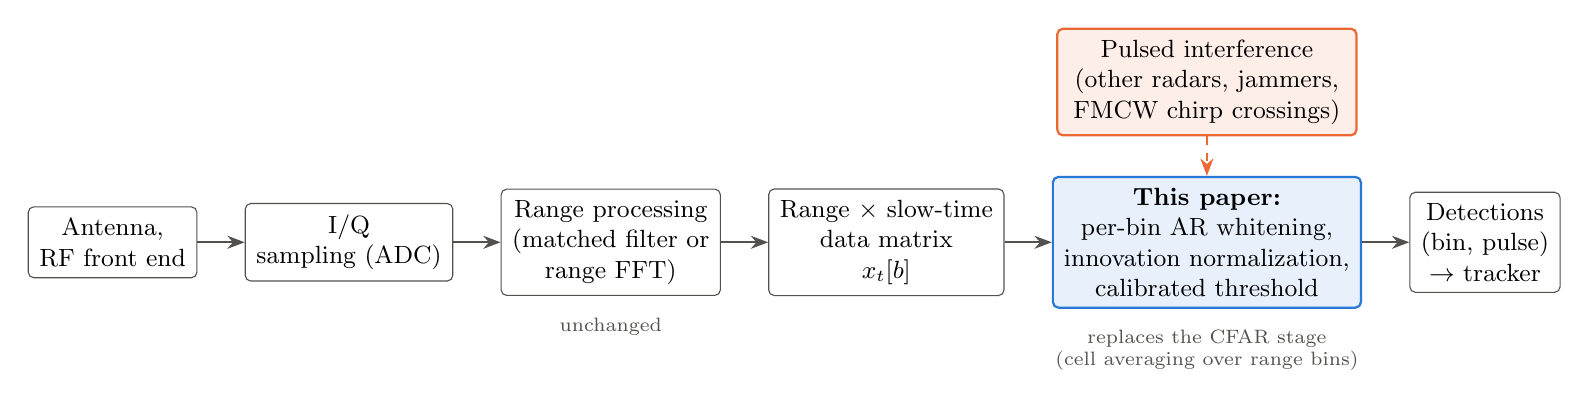
\begin{tikzpicture}[node distance=5mm and 6mm]
\node[blk] (rf) {Antenna,\\RF front end};
\node[blk,right=of rf] (adc) {I/Q\\sampling (ADC)};
\node[blk,right=of adc] (rng) {Range processing\\(matched filter or\\range FFT)};
\node[blk,right=of rng] (mat) {Range $\times$ slow-time\\data matrix\\$x_t[b]$};
\node[new,right=of mat,minimum width=38mm] (det) {\textbf{This paper:}\\per-bin AR whitening,\\innovation normalization,\\calibrated threshold};
\node[blk,right=of det] (out) {Detections\\(bin, pulse)\\$\to$ tracker};
\draw[arr] (rf)--(adc); \draw[arr] (adc)--(rng); \draw[arr] (rng)--(mat); \draw[arr] (mat)--(det); \draw[arr] (det)--(out);
\node[lab,below=1.5mm of det] {replaces the CFAR stage\\(cell averaging over range bins)};
\node[lab,below=1.5mm of rng] {unchanged};
\node[int,above=5mm of det,minimum width=38mm] (pi) {Pulsed interference\\(other radars, jammers,\\FMCW chirp crossings)};
\draw[arr,draw=acc2,dashed] (pi)--(det);
\end{tikzpicture}
\end{center}

\medskip
\noindent\textbf{(b) What happens to one range bin: the slow-time window of one test}\par\smallskip
\begin{center}
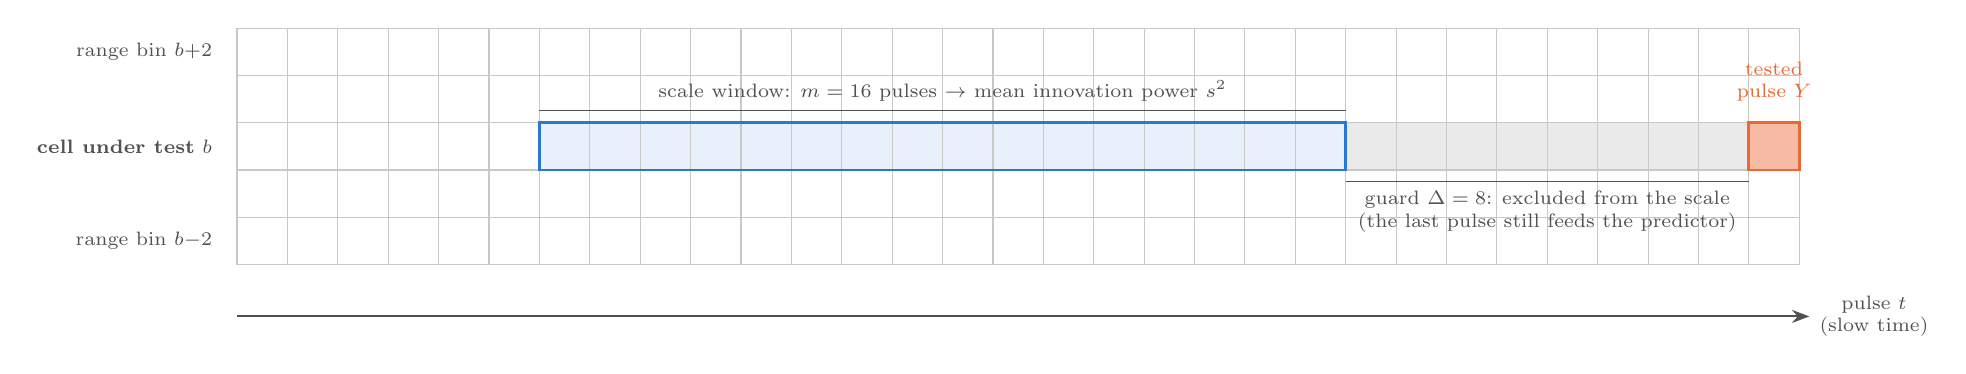
\begin{tikzpicture}[x=6.4mm,y=6mm]
\foreach \b in {0,...,4} {\foreach \t in {0,...,30} {\draw[grid,fill=white] (\t,\b) rectangle ++(1,1);}}
\fill[soft] (6,2) rectangle (22,3);
\fill[ink2!12] (22,2) rectangle (30,3);
\fill[acc2!45] (30,2) rectangle (31,3);
\foreach \t in {0,...,30} {\draw[grid] (\t,2) rectangle ++(1,1);}
\draw[acc,line width=1pt] (6,2) rectangle (22,3);
\draw[acc2,line width=1pt] (30,2) rectangle (31,3);
\node[lab,anchor=east] at (-0.3,4.5) {range bin $b{+}2$};
\node[lab,anchor=east] at (-0.3,2.5) {\textbf{cell under test} $b$};
\node[lab,anchor=east] at (-0.3,0.5) {range bin $b{-}2$};
\draw[ink2] (6,3.25)--(22,3.25); \node[lab,above] at (14,3.25) {scale window: $m=16$ pulses $\to$ mean innovation power $s^2$};
\draw[ink2] (22,1.75)--(30,1.75); \node[lab,below] at (26,1.75) {guard $\Delta=8$: excluded from the scale\\(the last pulse still feeds the predictor)};
\node[lab,text=acc2,above] at (30.5,3.25) {tested\\pulse $Y$};
\draw[arr] (0,-1.1)--(31.2,-1.1) node[right,lab] {pulse $t$\\(slow time)};
\end{tikzpicture}

\smallskip
{\small $\varepsilon_t=x_t-r\,x_{t-1}$ (AR(1) innovation; $r$ fitted on clutter training data), \quad score $=|\varepsilon_Y|^2/s^2$, \quad detection if score $>\widehat q^{\,2}$ (conformal threshold).}\\
{\small Without a guard, a target present for more than about four pulses enters the scale window and masks itself. With a guard of $\Delta$ pulses it stays visible for $\Delta$ more looks.}
\end{center}

\newpage
\noindent\textbf{(c) Inside the detector}\par\smallskip
\begin{center}
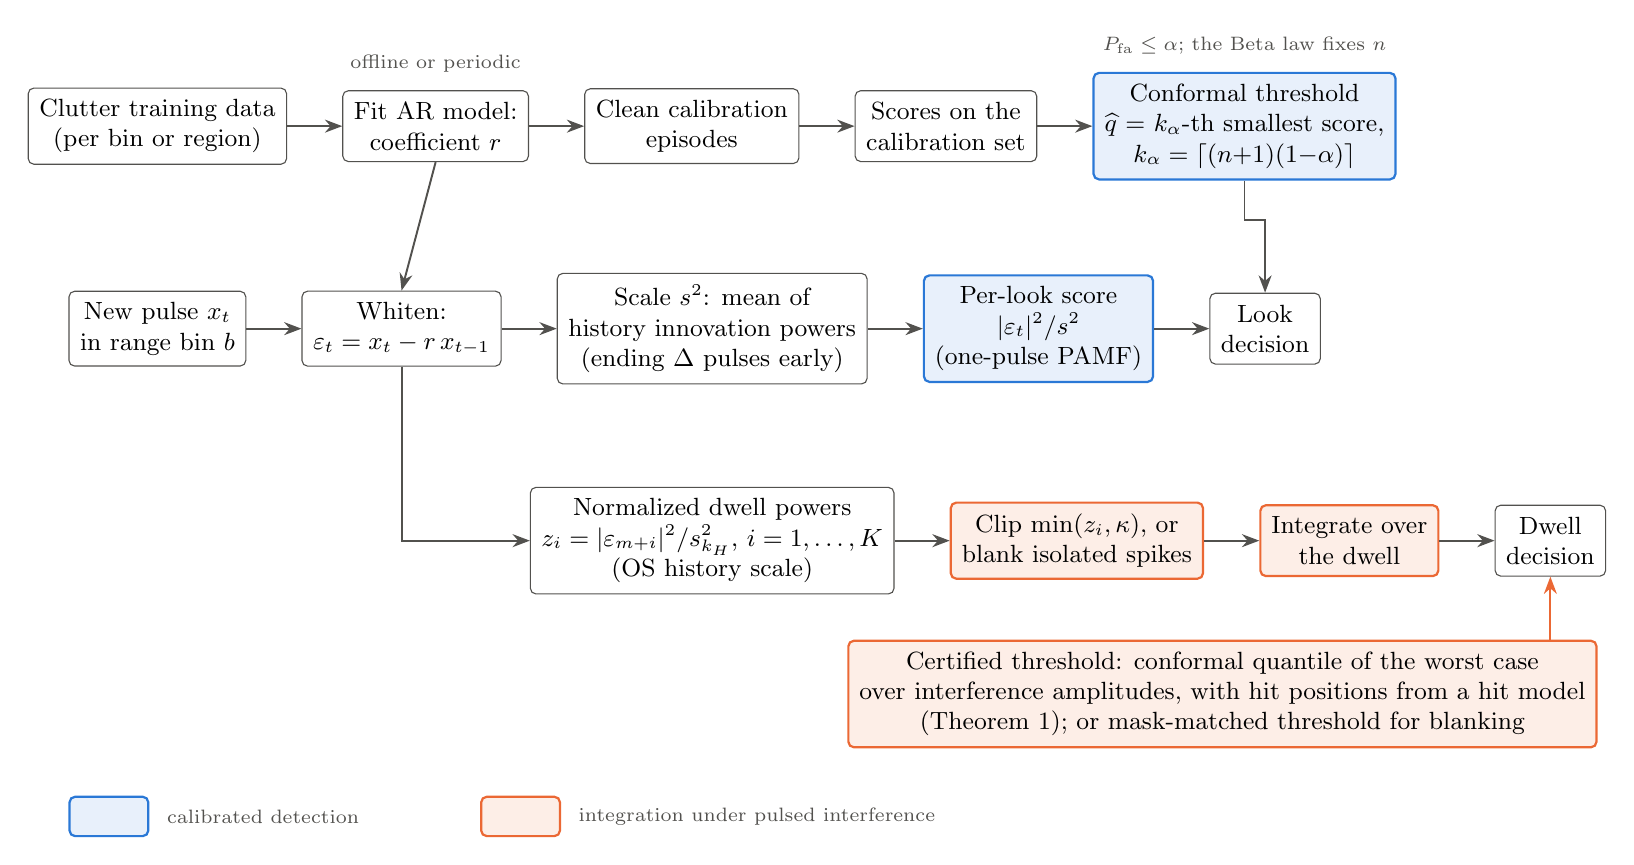
\begin{tikzpicture}[node distance=6mm and 7mm]
\node[blk] (tr) {Clutter training data\\(per bin or region)};
\node[blk,right=of tr] (fit) {Fit AR model:\\coefficient $r$};
\node[blk,right=of fit] (cal) {Clean calibration\\episodes};
\node[blk,right=of cal] (sc) {Scores on the\\calibration set};
\node[new,right=of sc] (q) {Conformal threshold\\$\widehat q$ = $k_\alpha$-th smallest score,\\$k_\alpha=\lceil(n{+}1)(1{-}\alpha)\rceil$};
\draw[arr] (tr)--(fit); \draw[arr] (fit)--(cal); \draw[arr] (cal)--(sc); \draw[arr] (sc)--(q);
\node[lab,above=1mm of fit] {offline or periodic};
\node[lab,above=1mm of q] {$P_{\rm fa}\le\alpha$; the Beta law fixes $n$};
% per-look lane
\node[blk,below=16mm of tr] (x) {New pulse $x_t$\\in range bin $b$};
\node[blk,right=of x] (w) {Whiten:\\$\varepsilon_t=x_t-r\,x_{t-1}$};
\node[blk,right=of w] (s) {Scale $s^2$: mean of\\history innovation powers\\(ending $\Delta$ pulses early)};
\node[new,right=of s] (pl) {Per-look score\\$|\varepsilon_t|^2/s^2$\\(one-pulse PAMF)};
\node[blk,right=of pl] (d1) {Look\\decision};
\draw[arr] (x)--(w); \draw[arr] (w)--(s); \draw[arr] (s)--(pl); \draw[arr] (pl)--(d1);
\draw[arr] (fit.south)--(w.north);
\draw[arr] (q.south) -- ++(0,-5mm) -| (d1.north);
% dwell lane
\node[blk,below=13mm of s] (z) {Normalized dwell powers\\$z_i=|\varepsilon_{m+i}|^2/s_{k_H}^2$, $i=1,\dots,K$\\(OS history scale)};
\node[int,right=of z] (clip) {Clip $\min(z_i,\kappa)$, or\\blank isolated spikes};
\node[int,right=of clip] (sum) {Integrate over\\the dwell};
\node[blk,right=of sum] (d2) {Dwell\\decision};
\draw[arr] (w.south) |- (z.west); \draw[arr] (z)--(clip); \draw[arr] (clip)--(sum); \draw[arr] (sum)--(d2);
\node[int,below=8mm of d2,anchor=north east,xshift=6mm] (cert) {Certified threshold: conformal quantile of the worst case\\over interference amplitudes, with hit positions from a hit model\\(Theorem 1); or mask-matched threshold for blanking};
\draw[arr,draw=acc2] (cert.north -| d2) -- (d2.south);
% legend
\node[new,minimum width=10mm,minimum height=5mm,anchor=north west] (lg1) at ($(x.west |- cert.south)+(0,-6mm)$) {};
\node[lab,right=1mm of lg1] {calibrated detection};
\node[int,right=42mm of lg1,minimum width=10mm,minimum height=5mm] (lg2) {};
\node[lab,right=1mm of lg2] {integration under pulsed interference};
\end{tikzpicture}
\end{center}

\medskip
\noindent\small\textbf{Reading the diagram.} Classical CA-CFAR estimates the noise level of the cell under test from neighbouring \emph{range} bins. That fails in sea clutter, whose strength (texture) changes from bin to bin. Here the reference is the cell's own \emph{past}. An AR filter first removes the pulse-to-pulse correlation of the clutter (whitening), and the tested innovation is then compared with the power of the past innovations, so the clutter's local strength cancels. The threshold is the $k_\alpha$-th smallest score on clean clutter (conformal), so it does not depend on a Gaussian model of the tail. A guard gap keeps a target that has just appeared out of the history. For dwell integration under pulsed interference, each normalized pulse power is clipped, or isolated spikes are blanked, before summation. The certified threshold bounds the false-alarm probability for interference of any power, provided the hit pattern is dominated by the hit model.
\end{document}
